\chapter{Thiết kế hệ thống truyền động}
\section{Thùng cấp liệu}
\begin{itemize}
    \item Vật liệu: Thép CT45
    \item Kích thước: 170x170x75 mm
    \item Tùy theo như cầu sử dụng mà có thể thay đổi kích thước của thùng cấp liệu cho phù hợp với yêu cầu của máy.
\end{itemize}
\begin{figure}[H]
    \centering
    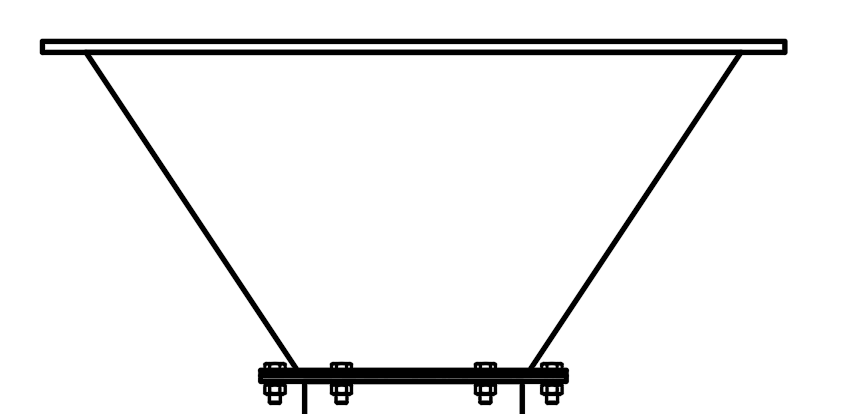
\includegraphics[width=0.5\textwidth]{pictures/thungcap.png}
\end{figure}

\section{Vít tải}
\begin{itemize}
    \item Vật liệu: Thép CT45
    \item Đường kính: 225 mm
    \item Tùy theo như cầu sử dụng mà có thể thay đổi kích thước của vít tải cho phù hợp với yêu cầu của máy.
\end{itemize}
\begin{figure}[H]
    \centering
    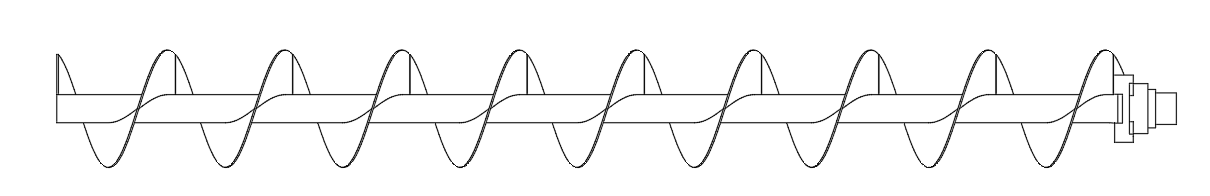
\includegraphics[width=1\textwidth]{pictures/vit.png}
\end{figure}

\section{Thân vít}
\begin{itemize}
    \item Vật liệu: Thép CT45
    \item Đường kính: 300 mm
    \item Thân vít được nối với thùng cấp liệu bằng bulong và đai ốc.
    \item Thân vít có chỗ xả liệu để xả bùn ra ngoài.
\end{itemize}
\begin{figure}[H]
    \centering
    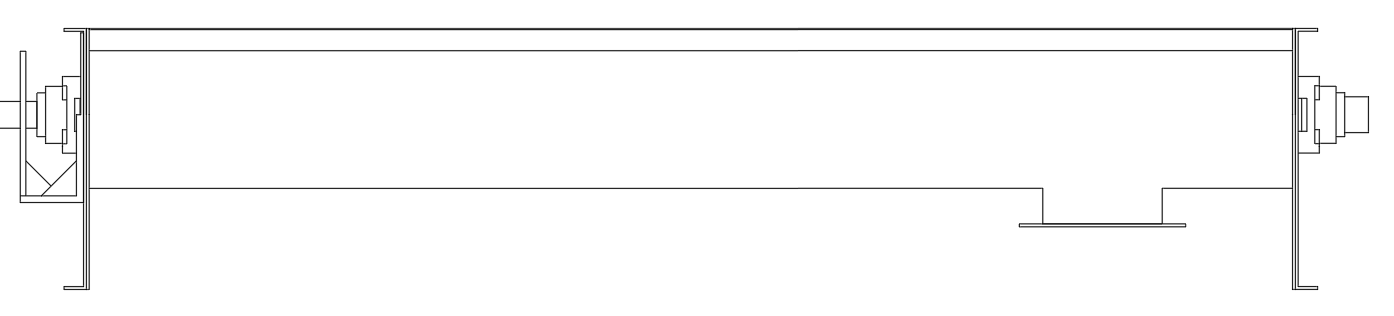
\includegraphics[width=1\textwidth]{pictures/than.png}
\end{figure}

\section{Bệ đỡ động cơ và hộp giảm tốc}
\begin{itemize}
    \item Vật liệu: Gang GX12-28.
    \item Cố định các đơn vị lắp lên bệ đỡ bằng bulong và đai ốc.
    \item Có thể sử dụng phương pháp hàn để cố định các bệ đỡ.
\end{itemize}
\begin{figure}[H]
    \centering
    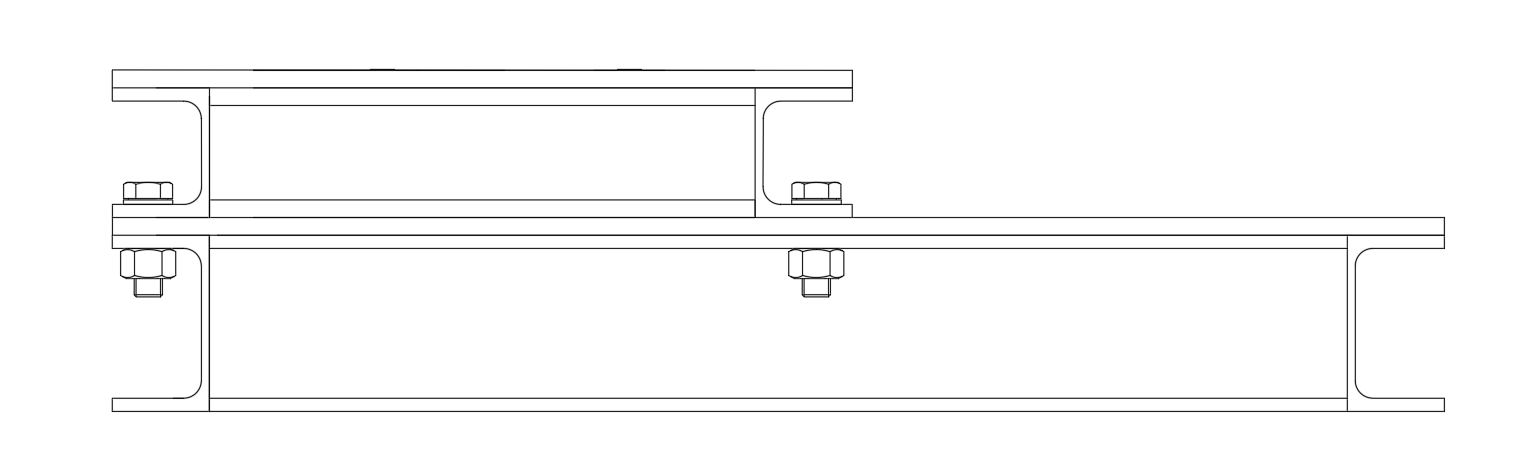
\includegraphics[width=1\textwidth]{pictures/be.png}
\end{figure}

\section{Bộ phận căng đai}
\begin{itemize}
    \item Chế tạo từ các tấm thép khi sản xuất đơn chiếc.
    \item Sử dụng gang xám khi sản xuất hàng loạt.
    \item Bộ phận căng đai được lắp trên bệ đỡ động cơ và hộp giảm tốc.
    \item Căng đai bằng phương pháp dịch chuyển động cơ tịnh tiến.
    \item Cố định với bệ đỡ và động cơ bằng bulong và đai ốc.
\end{itemize}
\begin{figure}[H]
    \centering
    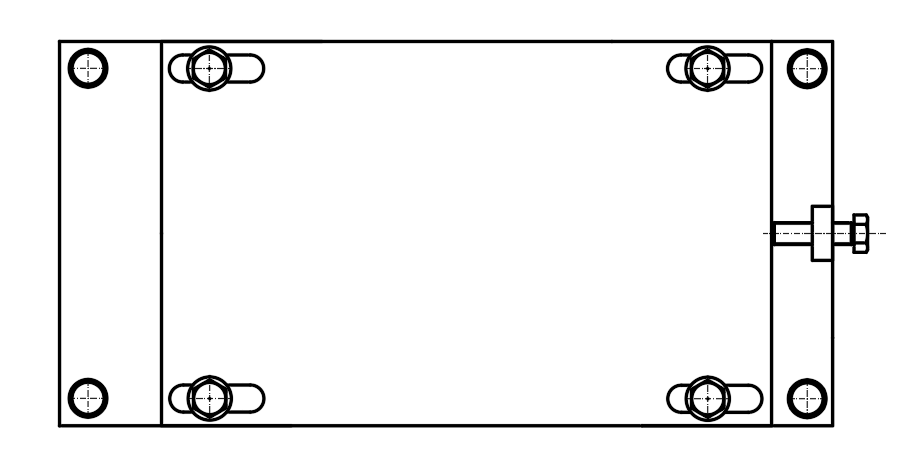
\includegraphics[width=1\textwidth]{pictures/cangdai.png}
\end{figure}